\section{Aufgabe 9}

In dieser Aufgabe sollte sich genauer mit der PDF, CDF und PPF der Exponentialverteilung befasst werden. Dafür muss die gegebene Funktion Zunächst
normiert werden. \\
Die Rechnung ist in Abbildung \ref{fig:normalize} zu finden.

\begin{figure}
    \centering
    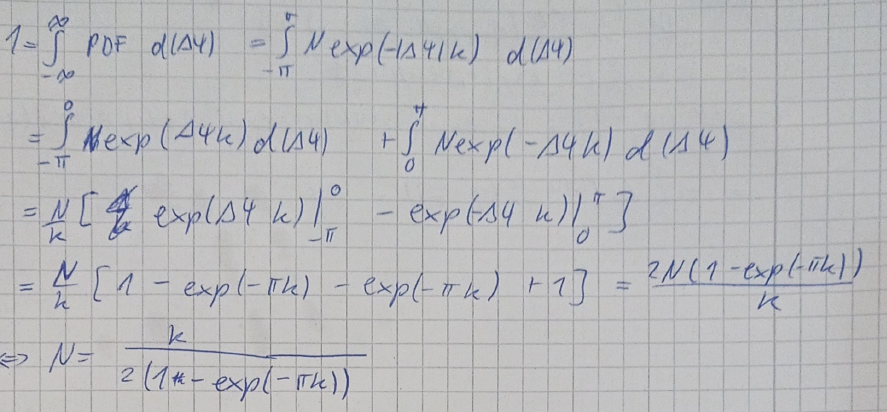
\includegraphics[width=\textwidth]{Norm.png}
    \caption{Normalisierung der PDF.}
    \label{fig:normalize}
\end{figure}
\FloatBarrier

\subsection{a)}
    Zunächst soll die PDF implementiert werden, dazu wird eine Fallunterscheidung verwendet. Es werden Masken verwendet,
    um die Werte des Datenarrays herauszusuchen, die in einen bestimmten Fall fallen, das heißt, die in das Intervall 
    $[-\pi, \pi)$ fallen.

\subsection{b)}
    Um die CDF zu erlangen wird die Formel
    \begin{equation*}
        \text{CDF} = \int_{-\infty}^{\increment \psi} \text{PDF}(\increment \psi) d\increment\psi 
    \end{equation*}
    verwendet. Dabei gibt es vier Fälle:
    \begin{itemize}
        \item Fall 1: $\increment\psi < -\pi$: CDF = 0, da die PDF auch null bis hier hin
        \item Fall 2: $-\pi < \increment \psi < 0$: $\text{CDF} = \int_{-\pi}^{\increment\psi} N \cdot \exp(\increment \psi \cdot k) d\increment\psi$
        \item Fall 3: $0 < \increment \psi < \pi$: $\text{CDF} = \int_{-\pi}^{0} N \cdot \exp(\increment \psi \cdot k) d\increment\psi + \int_{0}^{\increment\psi} N \cdot \exp(- \increment \psi \cdot k) d\increment\psi$
        \item Fall 4: $\increment \psi > \pi$: $\text{CDF} = 1$
    \end{itemize}
    In den Fällen 2 und 3 muss also noch integriert werden. Die entsprechenden Rechnungen sind in Abbildung \ref{fig:be} zu finden.
    
    \begin{figure}
        \centering
        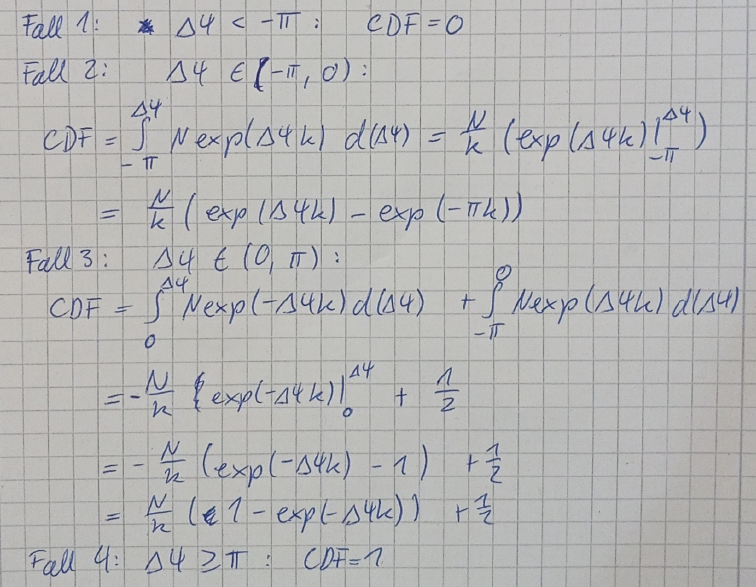
\includegraphics[width=\textwidth]{b.png}
        \caption{Berechnung der PDF.}
        \label{fig:be}
    \end{figure}
    \FloatBarrier

\subsection{c)}
    Die PPF ist die Inverse der CDF. Hier muss also intervallweise invertiert werden: für Wahrscheinlichkeiten zwischen 0 und 0.5 ist die PPF die Inverse des zweiten Falls 
    der CDF und für Wahrscheinlichkeiten zwischen 0.5 und 1 ist sie die Inverse des dritten Falls der CDF.\\
    Ist die Wahrscheinlichkeit null, kann die PPF auf $-\pi$ gesetzt werden während sie für 0.5 zu 0 wird und für 1 $\pi$. Die Rechnung ist in Abbildung zu finden. Erneut werden 
    Masken benutzt, um den Array aufzuteilen.

    \begin{figure}
        \centering
        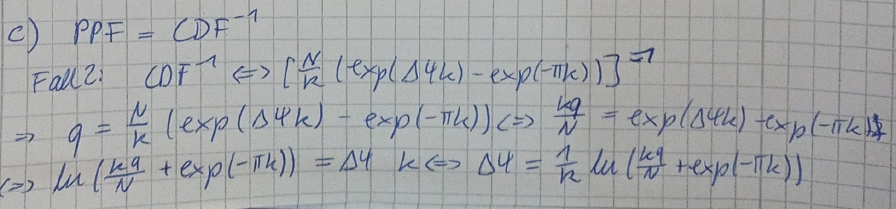
\includegraphics[width=\textwidth]{c1.png}
        \caption{Berechnung der PPF für $0 < q < 0.5$.}
        \label{fig:falleins}
    \end{figure}
    \FloatBarrier

    \begin{figure}
        \centering
        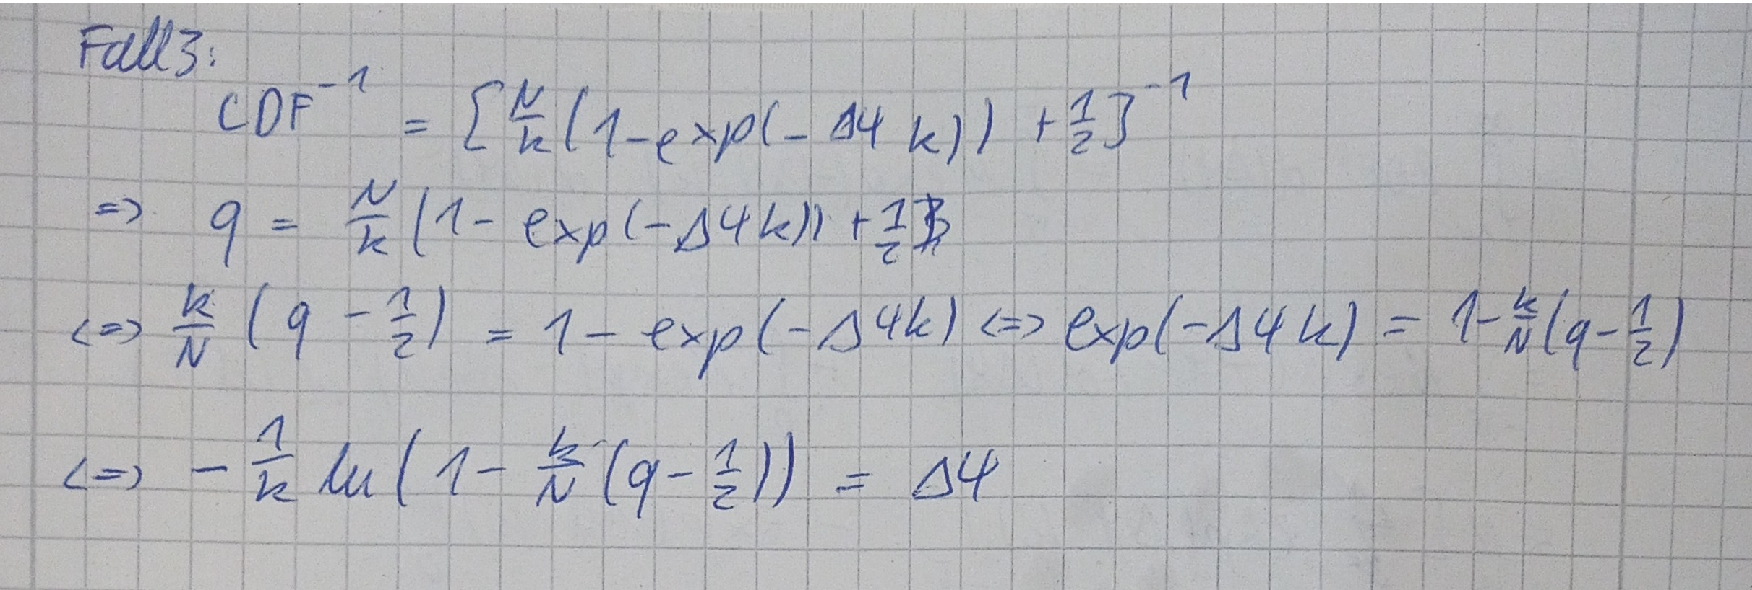
\includegraphics[width=\textwidth]{c2.pdf}
        \caption{Berechnung der PPF für $0.5 < q < 1$.}
        \label{fig:fallzwei}
    \end{figure}
    \FloatBarrier

\subsection{d)}
    Zum Schluss galt es, die implementierte PPF als random number generator zu verwenden, um eine Exponentialverteilung zu gewinnen. Gemäß des verfahrens werden dafür 
    zuerst gleichveteilte Zufallszahlen erzeugt, die dann als Argument der PPF übergeben werden. So ergibt sich die gesuchte Verteilung.\\
    \begin{figure}
        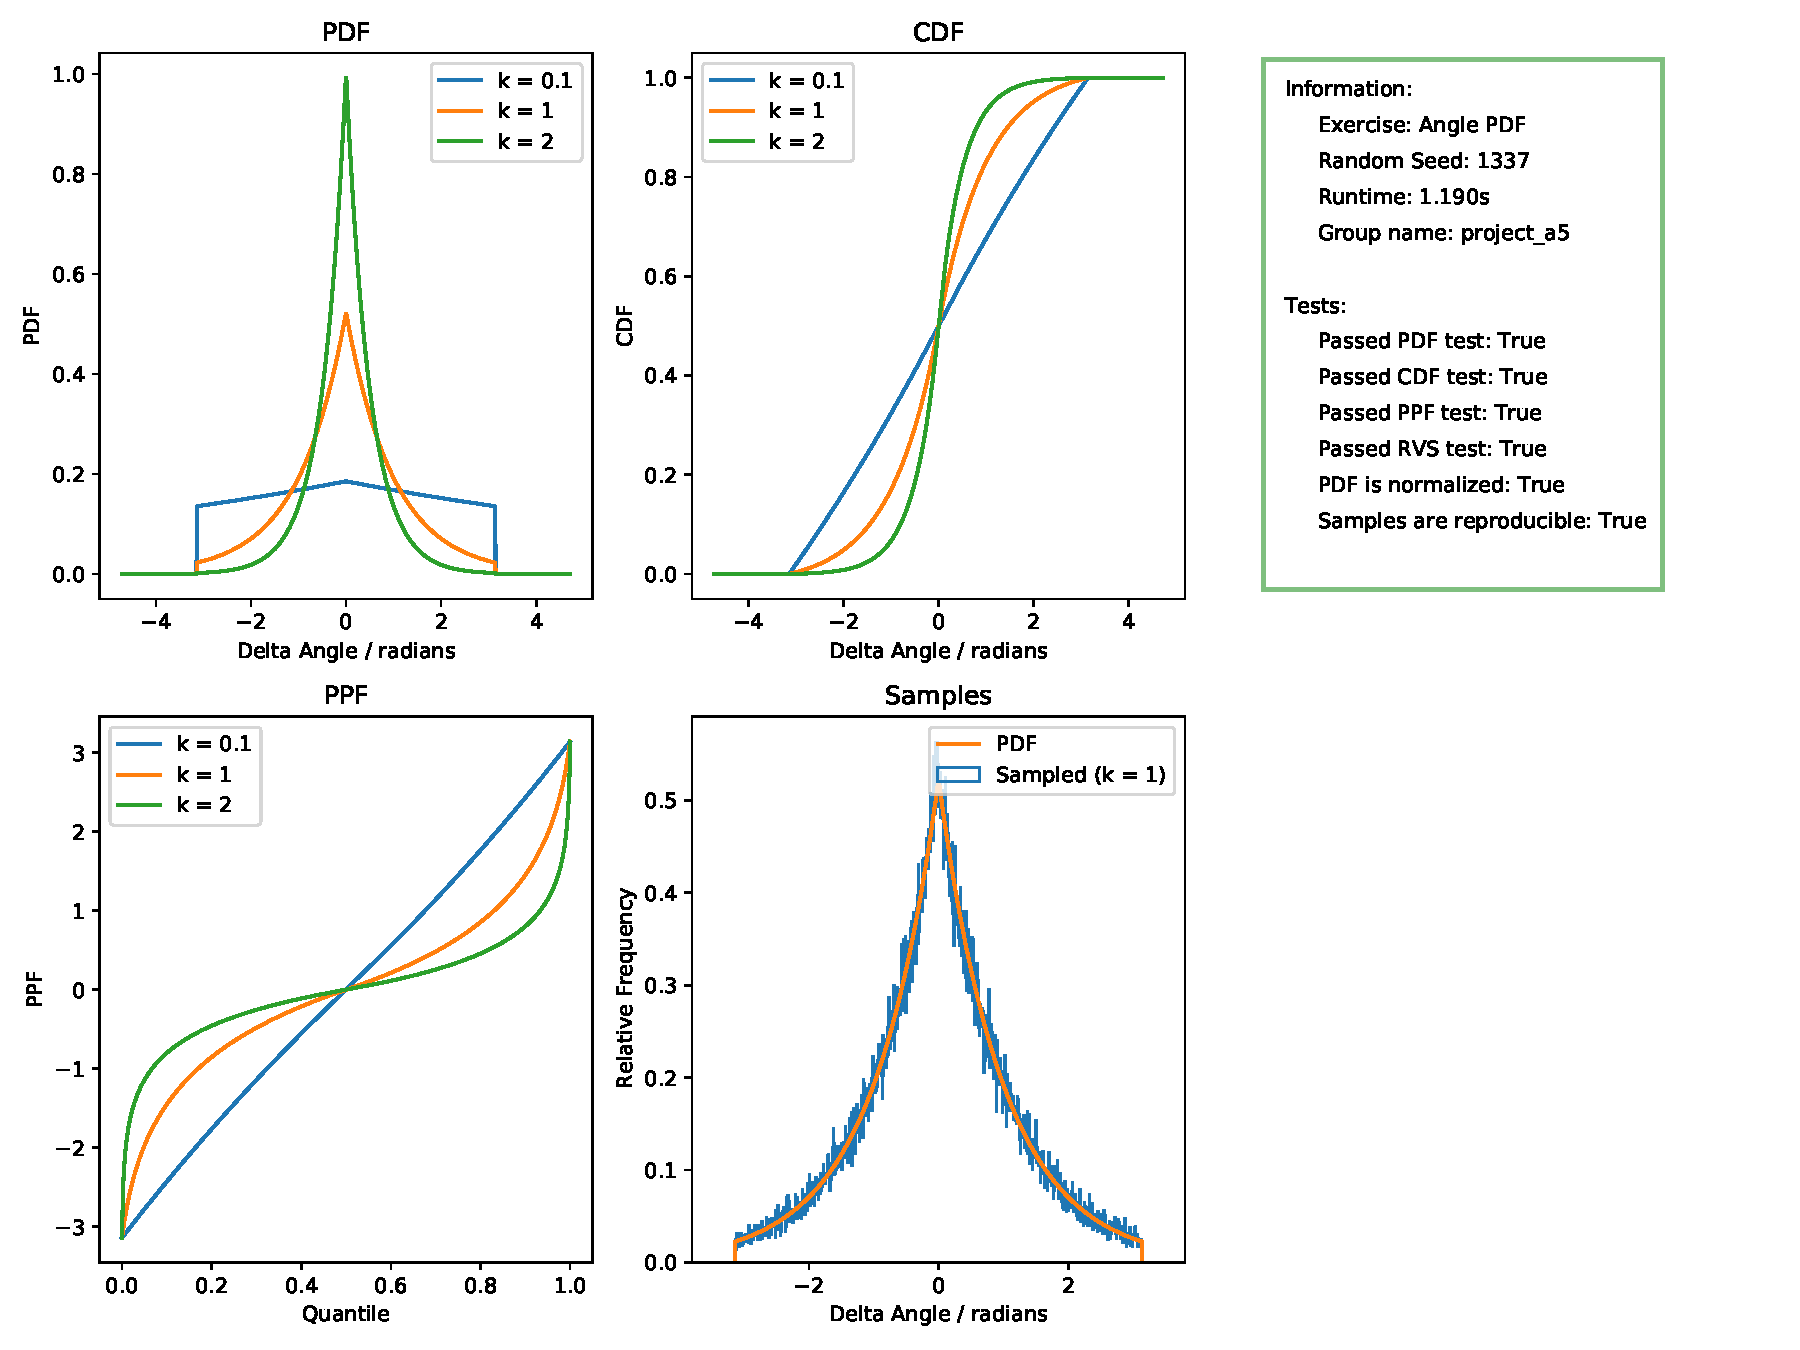
\includegraphics[width=\textwidth]{exercise_angle_pdf.pdf}
        \caption{Übersicht der Plots.}
        \label{fig:ubersicht}
    \end{figure}
    \FloatBarrier

    \noindent Es ist klar erkennbar, dass die erzeugten Zufallszahlen entlang der inversen kumulativen Verteilung verlaufen. 